\section{Hauptsatz} 
\subsection{Sprachen ohne optimales Beweissystem}

\begin{frame}
  \frametitle{Sprachen ohne optimales Beweissystem}
  
  \begin{theorem}
    Es gibt eine Sprache \(L \in \coNTIME(2^n)\), die kein optimales Beweissystem besitzt.
  \end{theorem}
\end{frame}

\subsection{Beweis}

\begin{frame}
  \frametitle{Beweisidee}

  \begin{enumerate}
   \item<1-> \(f_1, f_2, ...\): Aufzählung aller \(\FP\)-Funktionen
   \item<2-> \(L_i = 0^i10^*\) \\
              \onslide<3-> \(L_i'\) sind die Wörter aus \(L_i\), für die keine kurzen \(f_i\)-Beweise existieren \\
              \onslide<4-> \(L = \bigcup_i L_i' \in \coNTIME(2^n)\)
   \item<5-> \(L\)-Beweissystem \(f_i\): \(L_i' = L_i\), daher gibt es nur lange \(f_i\)-Beweise für \(L_i' \subset L\)
   \item<6-> Daher führt die Anname, dass \(f_i\) ein optimales Beweissystem für \(L\) ist, zum Widerspruch
  \end{enumerate}
\end{frame}

\begin{frame}
  \frametitle{Eine Aufzählung aller \(\FP\)-Funktionen}

  \begin{columns}
    \column{.7\textwidth}
      \begin{itemize}
        \item<2-> Gödel: \(M_1, M_2, ...\)
        \item<3-> \(M_1', M_2', ...\): \(M_i\) mit Wecker-Modifikation, sodass \(\runtime(M_i) \leq n^i + i\)
        \item<4-> \(f_i\): die von \(M_i\) berechnete Funktion
        \item<5-> \(n^i + i\) unbeschränkt, daher alle \(\FP\)-Funktionen
      \end{itemize}

    \column{.3\textwidth}
      \begin{figure}
        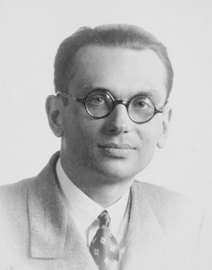
\includegraphics[width=\textwidth]{Presentation/Images/KurtGoedel.jpg}
        \caption{Kurt Gödel \\ 1906 -- 1978}
      \end{figure}
  \end{columns}
\end{frame}

\begin{frame}
  \frametitle{Konstruktion der gesuchten Sprache \(L\)}

  \begin{columns}
    \column{.2\textwidth}
      \begin{figure}
        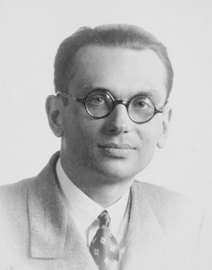
\includegraphics[width=\textwidth]{Presentation/Images/KurtGoedel.jpg}
        \caption{Kurt Gödel \\ 1906 -- 1978}
      \end{figure}

    \column{.8\textwidth}
      \begin{itemize}
        \item<1-> \(L_i = 0^i10^*\)
        \item<2-> Wähle \(x \in L_i'\), die keine kurzen \(f_i\)-Beweise haben
                  \[L_i' = \{ x \in L_i : \forall_{y \in \Sigma^*} |y|^{2i} \leq 2^{|x|} \implies f_i(y) \neq x \}\]
        \item<3-> Vereinigung
                  \[L = \bigcup_{i>0} L_i' \]
      \end{itemize}
  \end{columns}
\end{frame}

\begin{frame}
  \frametitle{\(L\) liegt in \(\coNTIME(2^n)\)}

  Betrachte Komplexität des Komplements
  
  \begin{itemize}
   \item<2-> \(L \in \coNTIME(2^n) \Leftrightarrow \overline{L} \in \NTIME(2^n)\)
   \item<3-> \(\overline{L} = \) \onslide<4-> \( \overline{ \bigcup_{i>0} L_i' } = \) \onslide<5-> \( \bigcap_{i>0} \overline{L_i'}\)
   \item<6-> zu zeigen: \( \bigcap_{i>0} \overline{L_i'} \in \NTIME(2^n)\)
  \end{itemize}

  \onslide<6->
  
  \(\overline{L_i'} = \{ x \in \Sigma^* : \alert<8-9>{ x \notin L_i } \vee \left( \alert<11>{ \exists_{y \in \Sigma^*} \left( |y|^{2i} \leq 2^{|x|} \right) } \wedge \alert<13>{ \left( f_i(y) = x \right) } \right)  \}\)

  \onslide<7-> Sei dazu \(x\) beliebiges Wort.

  \begin{itemize}
   \item<8-> Prüfe, ob \(x\) in irgendeinem \(L_i\): \onslide<9-> \alert<9>{falls nicht, dann \(x \in \overline{L}\) }
   \item<10-> Wählte \(i^*\) so, dass \(x \in L_{i^*}\)
   \item<11-> \alert<11>{für jedes \(y\) mit \(|y|^{2i} \leq 2^{|x|}\)}: \onslide<12-> berechne \(f_{i^*}(y)\). \onslide<13-> \alert<13>{Genau falls \(f_{i^*}(y) = x\), dann \(x \in \overline{L}\).}
  \end{itemize}

  \onslide<14>

  
\end{frame}


\begin{frame}
  \frametitle{Eigenschaft von \(L\)-Beweissystemen}

  Erinnerung: \(L_i' = \{ x \in L_i : \forall_{y \in \Sigma^*} |y|^{2i} \leq 2^{|x|} \implies f_i(y) \neq x \}\)
  
  \begin{itemize}
   \item<2-> jedes Beweissystem für \(L\) ist ein \(f_i\)
   \item<3-> für dieses ist \(L_i = L_i'\)
  \end{itemize}

  \begin{proof}
    \begin{itemize}
      \item<4-> angenommen, es gibt ein \(x = 0^i1z \in L_i\) das nicht in \(L_i'\) liegt
      \item<5-> dann gibt es \(y\) mit \(y^{2i} \leq 2^{|x|}\) und \(f_i(y) = x\)
      \item<6-> folglich \(x \in L_i'\) und daher \(x \in L\)
    \end{itemize}
  \end{proof}
\end{frame}

